% --- LaTeX Homework Template - S. Venkatraman ---

% --- Set document class and font size ---

\documentclass[letterpaper, 11pt]{article}

% --- Package imports ---

\usepackage{
  amsmath, amsthm, amssymb, mathtools, dsfont,	  % Math typesetting
  graphicx, wrapfig, subfig, float,                  % Figures and graphics formatting
  listings, color, inconsolata, pythonhighlight,     % Code formatting
  fancyhdr, sectsty, hyperref, enumerate, enumitem } % Headers/footers, section fonts, links, lists
  
  \usepackage{tikz}
  
  \tikzset{
  vtx/.style={circle, fill=black, inner sep=1.6pt},
  every picture/.style={>=latex}
}

\usetikzlibrary{positioning}

% --- Page layout settings ---

% Set page margins
\usepackage[left=0.7in, right=0.7in, bottom=1in, top=1.1in, headsep=0.2in]{geometry}

% Anchor footnotes to the bottom of the page
\usepackage[bottom]{footmisc}



% Set line spacing
\renewcommand{\baselinestretch}{1.2}

% Set spacing between paragraphs
\setlength{\parskip}{1.5mm}

% Allow multi-line equations to break onto the next page
\allowdisplaybreaks

% Enumerated lists: make numbers flush left, with parentheses around them
\setlist[enumerate]{wide=0pt, leftmargin=21pt, labelwidth=0pt, align=left}
\setenumerate[1]{label={(\arabic*)}}

% --- Page formatting settings ---

% Set link colors for labeled items (blue) and citations (red)
\hypersetup{colorlinks=true, linkcolor=blue, citecolor=red}

% Make reference section title font smaller
\renewcommand{\refname}{\large\bf{References}}

% --- Settings for printing computer code ---

% Define colors for green text (comments), grey text (line numbers),
% and green frame around code
\definecolor{greenText}{rgb}{0.5, 0.7, 0.5}
\definecolor{greyText}{rgb}{0.5, 0.5, 0.5}
\definecolor{codeFrame}{rgb}{0.5, 0.7, 0.5}

% Define code settings
\lstdefinestyle{code} {
  frame=single, rulecolor=\color{codeFrame},            % Include a green frame around the code
  numbers=left,                                         % Include line numbers
  numbersep=8pt,                                        % Add space between line numbers and frame
  numberstyle=\tiny\color{greyText},                    % Line number font size (tiny) and color (grey)
  commentstyle=\color{greenText},                       % Put comments in green text
  basicstyle=\linespread{1.1}\ttfamily\footnotesize,    % Set code line spacing
  keywordstyle=\ttfamily\footnotesize,                  % No special formatting for keywords
  showstringspaces=false,                               % No marks for spaces
  xleftmargin=1.95em,                                   % Align code frame with main text
  framexleftmargin=1.6em,                               % Extend frame left margin to include line numbers
  breaklines=true,                                      % Wrap long lines of code
  postbreak=\mbox{\textcolor{greenText}{$\hookrightarrow$}\space} % Mark wrapped lines with an arrow
}

% Set all code listings to be styled with the above settings
\lstset{style=code}

% --- Math/Statistics commands ---

% Add a reference number to a single line of a multi-line equation
% Usage: "\numberthis\label{labelNameHere}" in an align or gather environment
\newcommand\numberthis{\addtocounter{equation}{1}\tag{\theequation}}

% Shortcut for bold text in math mode, e.g. $\b{X}$
\let\b\mathbf

% Shortcut for bold Greek letters, e.g. $\bg{\beta}$
\let\bg\boldsymbol

% Shortcut for calligraphic script, e.g. %\mc{M}$
\let\mc\mathcal

% \mathscr{(letter here)} is sometimes used to denote vector spaces
\usepackage[mathscr]{euscript}

% Convergence: right arrow with optional text on top
% E.g. $\converge[w]$ for weak convergence
\newcommand{\converge}[1][]{\xrightarrow{#1}}

% Normal distribution: arguments are the mean and variance
% E.g. $\normal{\mu}{\sigma}$
\newcommand{\normal}[2]{\mathcal{N}\left(#1,#2\right)}

% Uniform distribution: arguments are the left and right endpoints
% E.g. $\unif{0}{1}$
\newcommand{\unif}[2]{\text{Uniform}(#1,#2)}

% Independent and identically distributed random variables
% E.g. $ X_1,...,X_n \iid \normal{0}{1}$
\newcommand{\iid}{\stackrel{\smash{\text{iid}}}{\sim}}

% Equality: equals sign with optional text on top
% E.g. $X \equals[d] Y$ for equality in distribution
\newcommand{\equals}[1][]{\stackrel{\smash{#1}}{=}}

% Math mode symbols for common sets and spaces. Example usage: $\R$
\newcommand{\R}{\mathbb{R}}   % Real numbers
\newcommand{\C}{\mathbb{C}}   % Complex numbers
\newcommand{\Q}{\mathbb{Q}}   % Rational numbers
\newcommand{\Z}{\mathbb{Z}}   % Integers
\newcommand{\N}{\mathbb{N}}   % Natural numbers
\newcommand{\F}{\mathcal{F}}  % Calligraphic F for a sigma algebra
\newcommand{\El}{\mathcal{L}} % Calligraphic L, e.g. for L^p spaces

% Math mode symbols for probability
\newcommand{\pr}{\mathbb{P}}    % Probability measure
\newcommand{\E}{\mathbb{E}}     % Expectation, e.g. $\E(X)$
\newcommand{\var}{\text{Var}}   % Variance, e.g. $\var(X)$
\newcommand{\cov}{\text{Cov}}   % Covariance, e.g. $\cov(X,Y)$
\newcommand{\corr}{\text{Corr}} % Correlation, e.g. $\corr(X,Y)$
\newcommand{\B}{\mathcal{B}}    % Borel sigma-algebra

% Other miscellaneous symbols
\newcommand{\tth}{\text{th}}	% Non-italicized 'th', e.g. $n^\tth$
\newcommand{\Oh}{\mathcal{O}}	% Big-O notation, e.g. $\O(n)$
\newcommand{\1}{\mathds{1}}	% Indicator function, e.g. $\1_A$

% Additional commands for math mode
\DeclareMathOperator*{\argmax}{argmax}    % Argmax, e.g. $\argmax_{x\in[0,1]} f(x)$
\DeclareMathOperator*{\argmin}{argmin}    % Argmin, e.g. $\argmin_{x\in[0,1]} f(x)$
\DeclareMathOperator*{\spann}{Span}       % Span, e.g. $\spann\{X_1,...,X_n\}$
\DeclareMathOperator*{\bias}{Bias}        % Bias, e.g. $\bias(\hat\theta)$
\DeclareMathOperator*{\ran}{ran}          % Range of an operator, e.g. $\ran(T) 
\DeclareMathOperator*{\dv}{d\!}           % Non-italicized 'with respect to', e.g. $\int f(x) \dv x$
\DeclareMathOperator*{\diag}{diag}        % Diagonal of a matrix, e.g. $\diag(M)$
\DeclareMathOperator*{\trace}{trace}      % Trace of a matrix, e.g. $\trace(M)$

% Numbered theorem, lemma, etc. settings - e.g., a definition, lemma, and theorem appearing in that 
% order in Section 2 will be numbered Definition 2.1, Lemma 2.2, Theorem 2.3. 
% Example usage: \begin{theorem}[Name of theorem] Theorem statement \end{theorem}
\theoremstyle{definition}
\newtheorem{theorem}{Theorem}[section]
\newtheorem{proposition}[theorem]{Proposition}
\newtheorem{lemma}[theorem]{Lemma}
\newtheorem{corollary}[theorem]{Corollary}
\newtheorem{definition}[theorem]{Definition}
\newtheorem{example}[theorem]{Example}
\newtheorem{remark}[theorem]{Remark}

% Un-numbered theorem, lemma, etc. settings
% Example usage: \begin{lemma*}[Name of lemma] Lemma statement \end{lemma*}
\newtheorem*{theorem*}{Theorem}
\newtheorem*{proposition*}{Proposition}
\newtheorem*{lemma*}{Lemma}
\newtheorem*{corollary*}{Corollary}
\newtheorem*{definition*}{Definition}
\newtheorem*{example*}{Example}
\newtheorem*{remark*}{Remark}
\newtheorem*{claim}{Claim}
\newcommand{\Tau}{\mathcal{T}}
\newcommand{\PSet}{\mathcal{P}}





% --- Left/right header text (to appear on every page) ---

% Include a line underneath the header, no footer line
\pagestyle{fancy}
\renewcommand{\footrulewidth}{0pt}
\renewcommand{\headrulewidth}{0.4pt}

% Left header text: course name/assignment number
\lhead{MAM4000W, Graph Theory -- Chapter 3 Problems}

% Right header text: your name
\rhead{Alex Cristaudo, CRSALE010}

% --- Document starts here ---

\begin{document}

\subsection*{Question 1: Prove Theorem 3.1.3: A non-trivial connected graph $G$ has an eulerian circuit if and only if every vertex of $G$ has even degree}
$(\Longrightarrow)$ Assume that $G$ has an Eulerian circuit $v_0,v_1,...,v_k,v_0$. For every $1 \le i \le k$, the occurence of a vertex $v_i$ involves adding 2 edges to its degree, namely $v_{i-1}v_i$ and $v_iv_{i+1}$. Since every edge is unique, we will always add 2. For vertex $v_0$, we have edges $v_0v_1$ and $v_{k}v_0$, an even amount.After this, every edge has been counted and it follows every vertex has even degree. \\
$(\Longleftarrow)$ We strong induct on the size of $G = m$. The case when $m = 2$ is trivial. (bounce back and forth between the vertices using each edge once). [Or we can use the trivial graph as the base case for $m=0$] Assume we can find a Euclerian circuit for any graph of size less than $m$. Now let $G$ be a graph of size $m$. If $G$ is acyclic (since it is connected), it is a tree and thus has at least 2 end-vertices, a contradiction. So $G$ is cyclic and has a cycle $C: w_1w_2w_3...w_k$. Consider the components after cutting edges $\{w_1w_2, w_2w_3, ..., w_kw_1\}$ being $C_1, ..., C_N$. Each of these components has size less than $m$, and even degrees (as only the cycle vertices are affected, each removing 2 degrees) and are connected to cycle $C$ by some vertex $w_i$. By the inductive hypothesis, so have Euclerian circuits $P_i$. We construct a Euclerian path as follows: Proceed along cycle $C$. If I come across some vertex on $C$ in $C_i$, use path $P_i$ unless that path has been processed already, then just move to the next vertex on $C$. This new circuit is Euclerian as required.

\subsection*{Question 2: Prove Theorem 3.1.4: A non-trivial connected $G$ has an Euclerian trail if and only if $G$ contains exactly two vertices of odd degree. Furthermore, every Euclerian trail begins at one of these odd vertices and ends at the other}

We can prove it similarly as to how we did in Question 1, but a shorter way is to modify graph $G$ into $H$ by adding one edge between these odd vertices (call them $u$ and $v$). Then $G$ has exactly 2 odd vertices if and only if $H$ has even vertices if and only if $H$ has a Euclerian circuit. Now if $P: v_0...v_{i-1}uvv_i...v_kv_0$ is a Euclerian circuit for $H$, then $vv_i...v_kv_0v_1...v_{i-1}u$ is an Eulerian trail (in $G$) starting and ending at these odd vertices. On the other hand, if $uv_0v_1...v_{i-1}v_i...v_kv$ is an Eulerian trail starting and ending at these odd vertices (in $G$), then $vuv_0v_1...v_kv$ is an Eulerian circuit in $H$. So We have an Eulerian trail in $G$ starting and ending at these odd vertices if and only if we have an Eulerian circuit in $H$. Finally, we get $G$ has an Eulerian trail starting and ending at these odd vertices if and only exactly 2 vertices have odd degree. Clearly Every Eulerian trail in $G$ must start and end at these odd vertices, by the degree argument above if they start somewhere else these odd vertices have even degree.

\newpage

\subsection*{Question 3: Prove that the converse of Theorem 3.2.3 is not true: Show that for a graph $G$, if every proper non-empty subset $S \subseteq V(G)$, we have $k(G-S) \le |S|$, then $G$ is Hamiltonian is false. }

\begin{figure}[h]
\centering
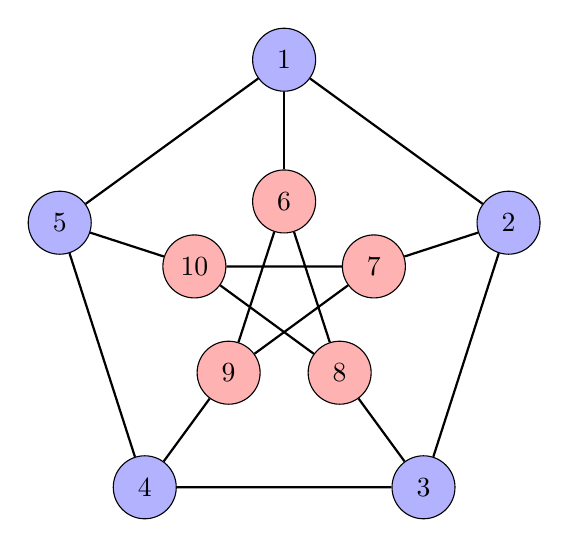
\begin{tikzpicture}[scale=1.5]
    % Outer pentagon vertices
    \node[circle, fill=blue!30, draw, minimum size=8mm] (O1) at (0,2) {1};
    \node[circle, fill=blue!30, draw, minimum size=8mm] (O2) at (1.9,0.62) {2};
    \node[circle, fill=blue!30, draw, minimum size=8mm] (O3) at (1.18,-1.62) {3};
    \node[circle, fill=blue!30, draw, minimum size=8mm] (O4) at (-1.18,-1.62) {4};
    \node[circle, fill=blue!30, draw, minimum size=8mm] (O5) at (-1.9,0.62) {5};
    
    % Inner pentagram vertices
    \node[circle, fill=red!30, draw, minimum size=8mm] (I1) at (0,0.8) {6};
    \node[circle, fill=red!30, draw, minimum size=8mm] (I2) at (0.76,0.25) {7};
    \node[circle, fill=red!30, draw, minimum size=8mm] (I3) at (0.47,-0.65) {8};
    \node[circle, fill=red!30, draw, minimum size=8mm] (I4) at (-0.47,-0.65) {9};
    \node[circle, fill=red!30, draw, minimum size=8mm] (I5) at (-0.76,0.25) {10};
    
    % Outer pentagon edges
    \draw[thick] (O1) -- (O2) -- (O3) -- (O4) -- (O5) -- (O1);
    
    % Inner pentagram edges (connecting every other vertex)
    \draw[thick] (I1) -- (I3) -- (I5) -- (I2) -- (I4) -- (I1);
    
    % Spokes connecting outer to inner
    \draw[thick] (O1) -- (I1);
    \draw[thick] (O2) -- (I2);
    \draw[thick] (O3) -- (I3);
    \draw[thick] (O4) -- (I4);
    \draw[thick] (O5) -- (I5);
    
\end{tikzpicture}
\caption{The Petersen Graph}
\label{fig:petersen}
\end{figure}
~\\
The Petersen Graph $G$ is not Hamiltonian and $\kappa (G) = 3$ so for $|S| < 3$ clearly $k(G-S) \le |S|$. If we think of how to split $G$ into 3 components, it involves removing 5 vertices (isolating 2 outer vertices). This is clearly the minimum since for any $u,v,w \in V(G)$, $p(u,v) = p(v,w) = 3$ and there is only one $u-w$ path passing through $v$. (Each path must remove a vertex to separate them into 3 components, with only one vertex being shared along other paths). Creating 4 components is impossible since if we want 4 vertices in different components, pick one vertex. This has 3 neighbours that cant be the other vertices. This leaves 6 other vertices. Picking another vertex also has 3 neighbours, with at most 1 shared with vertex 1. This leaves 3 vertices for 2 other selections, impossible as each vertex will guarantee at least 2 more vertices we cannot pick. A simpler graph is simply the disconnected graph with 2 vertices.

\subsection*{Question 4: Prove Corollary 3.2.5: Let $u$ and $v$ be distinct non-adjacent vertices of a graph $G$ of order $n$ such that $\deg u + \deg v \ge n$. Then $G$ is Hamiltonian if and only if $G + uv$ is Hamiltonian}
Clearly if $G$ is Hamiltonian, then so is $G + uv$ (the Hamiltonian cycle for $G$ is also a Hamiltonian cycle for $G + uv$). So suppose that $G + uv$ is Hamiltonian. Let $P: v_0v_1...v_kv_0$ be a Hamiltonian cycle. If edge $uv$ is not used, we are done and this is a Hamiltonian cycle for $G$. Otherwise $P : v_0v_1...v_{i}uvv_{i+1}...v_0$ means $vv_{i+1}...v_kv_0v_1...v_{i}u := vw_0w_1...w_{k-2}u$ is a Hamiltonian path. Since $\deg u + \deg v \ge n$, and there are $n-2$ other vertices, there are at least two vertices $w_i$ and $w_j$ neighbouring both (and all other vertices neighbour one). Without loss of generality, assume $i < j$. First suppose $i + 1 \ne j$. If $w_{i+1}$ neighbours $v$, we get Hamiltonian cycle $w_j ...w_{i+1}vw_0...w_iuw_{k-2}...w_j$. If $w_{j-1}$ neighbours $u$, we get Hamiltonian cycle $w_i ... w_{j-1}uw_{k-2}...w_j v w_0 ... w_i$. So assuming neither of those cases hold, we can look at whether $w_{i+2}$ neighbours $v$ or $w_{j-2}$ neighbours $u$. Again, in these cases we find Hamiltonian cycles similarly. Again, assuming these dont happen, we can continue working inwards and we will eventually find a pair that satisfies this (otherwise we get a contradiction when $j - N < i + N$). Whats left is to check the case when $j = i + 1$. This is simple, we use Hamiltonian cycle $vw_0...w_iuw_{k-2}...w_{j}v$.

 ~\\Using the fact it is a Corollary, we follow a similar proof that they did. 
Clearly if $G$ is Hamiltonian, then so is $G + uv$. Suppose there is a graph $G$ that is not Hamiltonian, but $G + uv$ is. Let $C$ be a Hamiltonian cycle of $G+uv$. Necessarily, the edge $uv$ lies on $C$, so there is a $u-v$ path $P:u=u_1,u_2,...,u_n=v$ that contains every vertex of $G$. If $u_1u_i \in E(G)$, then necessarily $u_{i-1}u_n \notin E(G)$, for otherwise $u_1,u_2,...,u_{i-1}u_n,u_{n-1},...,u_i,u_1$ is a Hamiltonian cycle of $G$. Consequently, $\deg (u_n) \le n-1-\deg u_1$. So $\deg u + \deg v \le n-1$, a contradiction.

\subsection*{Question 5: Let $G_1$ and $G_2$ be two Eulerian graphs with no vertex in common. Let $v_1 \in V(G_1)$ and $v_2 \in V(G_2)$. Let $G$ be the graph obtained from $G_1 \cup G_2$ by adding the edge $v_1v_2$. What can be said about $G$?}

$G$ has an Eulerian trail. In $G_1$ and $G_2$, every vertex has even degree (from the graphs being Eulerian). Adding edge $v_1v_2$ in $G$ means $v_1$ and $v_2$ have odd degrees. $G_1$ and $G_2$ share no vertices, so only $v_1$ and $v_2$ have odd degrees and thus $G$ has an Eulerian trail.

\newpage
\subsection*{Question 6: Give an example of a graph $G$ such that:}
\subsubsection*{\ \ (a) both $G$ and $\bar{G}$ are Eulerian}

\begin{figure}[h]\centering
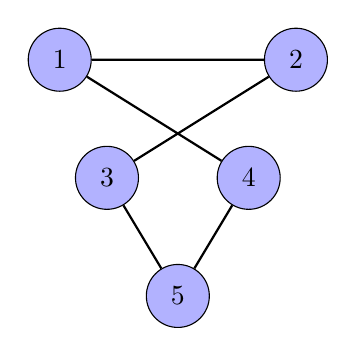
\begin{tikzpicture}[scale=1.5]
    % Vertices
    \node[circle, fill=blue!30, draw, minimum size=8mm] (1) at (-1,1) {1};
    \node[circle, fill=blue!30, draw, minimum size=8mm] (2) at ( 1,1) {2};
    \node[circle, fill=blue!30, draw, minimum size=8mm] (3) at (-0.6,0) {3};
    \node[circle, fill=blue!30, draw, minimum size=8mm] (4) at ( 0.6,0) {4};
    \node[circle, fill=blue!30, draw, minimum size=8mm] (5) at ( 0,-1) {5};
    % Edges (5-cycle)
    \draw[thick] (1)--(4)--(5)--(3)--(2)--(1);
\end{tikzpicture}
\end{figure}

\subsubsection*{\ \ (b) $G$ is Eulerian but $\bar{G}$ is not}
% (b) C4
\begin{figure}[h]\centering
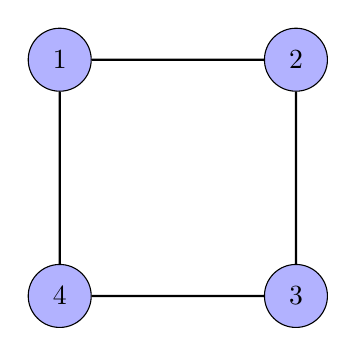
\begin{tikzpicture}[scale=1.5]
    \node[circle, fill=blue!30, draw, minimum size=8mm] (1) at (-1,1) {1};
    \node[circle, fill=blue!30, draw, minimum size=8mm] (2) at ( 1,1) {2};
    \node[circle, fill=blue!30, draw, minimum size=8mm] (3) at ( 1,-1) {3};
    \node[circle, fill=blue!30, draw, minimum size=8mm] (4) at (-1,-1) {4};
    \draw[thick] (1)--(2)--(3)--(4)--(1);
\end{tikzpicture}
\end{figure}

\subsubsection*{\ \ (c) both $G$ and $\bar{G}$ contain an Eulerian trail}
\begin{figure}[h]\centering
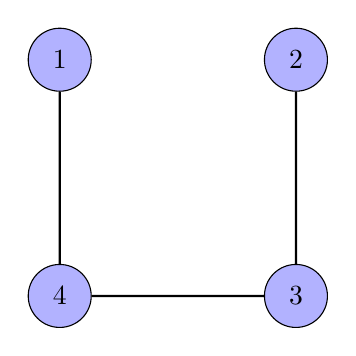
\begin{tikzpicture}[scale=1.5]
    \node[circle, fill=blue!30, draw, minimum size=8mm] (1) at (-1,1) {1};
    \node[circle, fill=blue!30, draw, minimum size=8mm] (2) at ( 1,1) {2};
    \node[circle, fill=blue!30, draw, minimum size=8mm] (3) at ( 1,-1) {3};
    \node[circle, fill=blue!30, draw, minimum size=8mm] (4) at (-1,-1) {4};
    \draw[thick] (2)--(3)--(4)--(1);
\end{tikzpicture}
\end{figure}

\newpage

\subsubsection*{\ \ (d) $G$ contains an Eulerian trail and an edge $e$ such that $G-e$ is Eulerian}
\begin{figure}[h]\centering
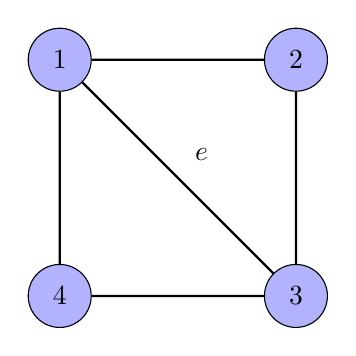
\begin{tikzpicture}[scale=1.5]
    \node[circle, fill=blue!30, draw, minimum size=8mm] (1) at (-1,1) {1};
    \node[circle, fill=blue!30, draw, minimum size=8mm] (2) at ( 1,1) {2};
    \node[circle, fill=blue!30, draw, minimum size=8mm] (3) at ( 1,-1) {3};
    \node[circle, fill=blue!30, draw, minimum size=8mm] (4) at (-1,-1) {4};
    \draw[thick] (1)--(2)--(3)--(4)--(1);
    \draw[thick] (1)--(3);
    
    \node at (0.2,0.2) {$e$};
\end{tikzpicture}
\end{figure}

\subsubsection*{\ \ (e) $G$ is Eulerian but not Hamiltonian}
\begin{figure}[h]\centering
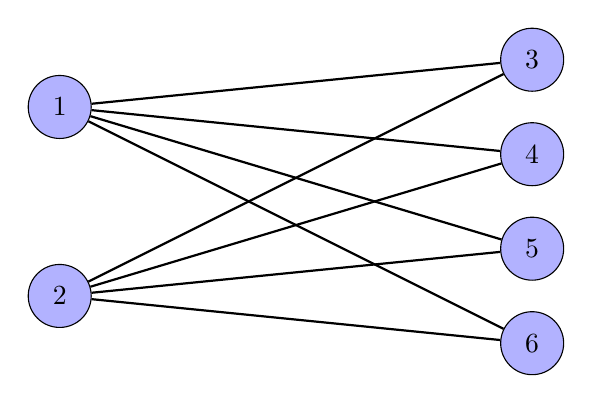
\begin{tikzpicture}[scale=1.5]
    % Left part (2 vertices)
    \node[circle, fill=blue!30, draw, minimum size=8mm] (L1) at (-2, 0.8) {1};
    \node[circle, fill=blue!30, draw, minimum size=8mm] (L2) at (-2,-0.8) {2};
    % Right part (4 vertices)
    \node[circle, fill=blue!30, draw, minimum size=8mm] (R1) at ( 2, 1.2) {3};
    \node[circle, fill=blue!30, draw, minimum size=8mm] (R2) at ( 2, 0.4) {4};
    \node[circle, fill=blue!30, draw, minimum size=8mm] (R3) at ( 2,-0.4) {5};
    \node[circle, fill=blue!30, draw, minimum size=8mm] (R4) at ( 2,-1.2) {6};
    % Edges
    \foreach \L in {L1,L2}{
        \foreach \R in {R1,R2,R3,R4}{
            \draw[thick] (\L)--(\R);
        }
    }
\end{tikzpicture}
\end{figure}

\subsubsection*{\ \ (f) $G$ is Hamiltonian but not Eulerian}
\begin{figure}[h]\centering
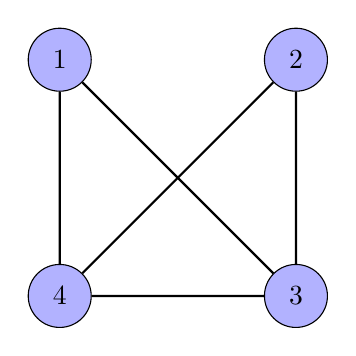
\begin{tikzpicture}[scale=1.5]
    \node[circle, fill=blue!30, draw, minimum size=8mm]  (1) at (-1,1) {1};
    \node[circle, fill=blue!30, draw, minimum size=8mm]  (2) at ( 1,1) {2};
    \node[circle, fill=blue!30, draw, minimum size=8mm]  (3) at ( 1,-1) {3};
    \node[circle, fill=blue!30, draw, minimum size=8mm]  (4) at (-1,-1) {4};
    % Outer edges minus (1,2)
    \draw[thick] (2)--(3)--(4)--(1);
    % Diagonals
    \draw[thick] (1)--(3);
    \draw[thick] (2)--(4);
\end{tikzpicture}
\end{figure}

\newpage

\subsubsection*{\ \ (g) $G$ is Hamiltonian and has an Eulerian trail}
\begin{figure}[h]\centering
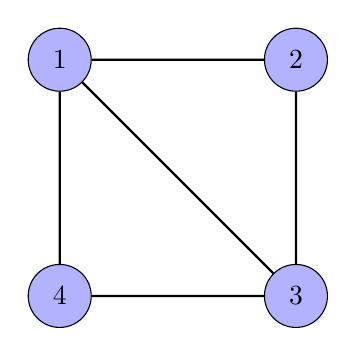
\begin{tikzpicture}[scale=1.5]
    \node[circle, fill=blue!30, draw, minimum size=8mm]  (1) at (-1,1) {1};
    \node[circle, fill=blue!30, draw, minimum size=8mm]  (2) at ( 1,1) {2};
    \node[circle, fill=blue!30, draw, minimum size=8mm]  (3) at ( 1,-1) {3};
    \node[circle, fill=blue!30, draw, minimum size=8mm]  (4) at (-1,-1) {4};
    \draw[thick] (1)--(2)--(3)--(4)--(1);
    \draw[thick] (1)--(3);
\end{tikzpicture}
\end{figure}

\subsubsection*{\ \ (h) $G$ is not Hamiltonian and $G$ has an Eulerian trail}
\begin{figure}[h]\centering
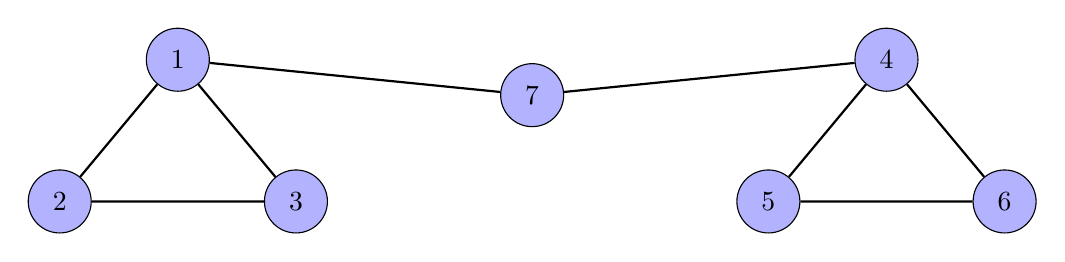
\begin{tikzpicture}[scale=1.5]
    % Left triangle
    \node[circle, fill=blue!30, draw, minimum size=8mm]  (L1) at (-3, 0) {1};
    \node[circle, fill=blue!30, draw, minimum size=8mm]  (L2) at (-4,-1.2) {2};
    \node[circle, fill=blue!30, draw, minimum size=8mm]  (L3) at (-2,-1.2) {3};
    \draw[thick] (L1)--(L2)--(L3)--(L1);
    % Right triangle
    \node[circle, fill=blue!30, draw, minimum size=8mm]  (R1) at ( 3, 0) {4};
    \node[circle, fill=blue!30, draw, minimum size=8mm]  (R2) at ( 2,-1.2) {5};
    \node[circle, fill=blue!30, draw, minimum size=8mm]  (R3) at ( 4,-1.2) {6};
    \draw[thick] (R1)--(R2)--(R3)--(R1);
    % Cut vertex
    \node[circle, fill=blue!30, draw, minimum size=8mm]  (X) at (0,-0.3) {7};
    \draw[thick] (X)--(L1);
    \draw[thick] (X)--(R1);
\end{tikzpicture}
\end{figure}

\subsection*{Question 7: Show that every nontrivial connected graph has a closed spanning walk that contains every edge exactly twice}
Modify our graph $G$ into a non-simple graph $H$, where every edge is duplicated once. Then $H$ has even degree and thus has a Euclerian circuit. This is equivalent to $G$ having a closed spanning walk that contains every edge exactly twice.
\newpage

\subsection*{Question 8: Prove or disprove:}
\subsubsection*{\ \ (a) If $G$ is 2-connected, then $G$ is Hamiltonian}
This is not true. Consider graph: (or Petersen graph)
\begin{figure}[h]\centering
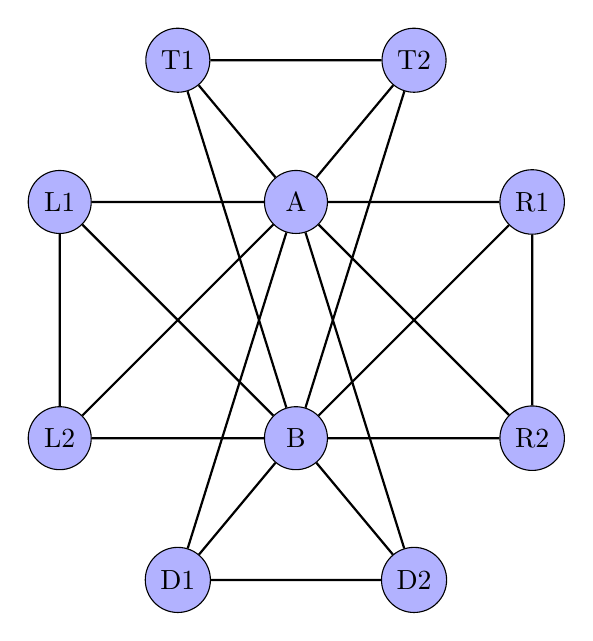
\begin{tikzpicture}[scale=1.5,
  every node/.style={circle, fill=blue!30, draw, minimum size=8mm}]

  % Central shared vertices
  \node (A) at (0,1) {A};
  \node (B) at (0,-1) {B};

  % Extra vertices for left K4
  \node (L1) at (-2,1) {L1};
  \node (L2) at (-2,-1) {L2};

  % Extra vertices for right K4
  \node (R1) at ( 2,1) {R1};
  \node (R2) at ( 2,-1) {R2};

  % Top K3 vertex
  \node (T1) at (-1,2.2) {T1};
  \node (T2) at (1,2.2) {T2};

  % Bottom K3 vertex
  \node (D1) at (-1,-2.2) {D1};
    \node (D2) at (1,-2.2) {D2};

  %--- Edges ---
  % Left K4 (A,B,L1,L2), but missing edge between A and B’s "opposite side" (so remove L1--L2?)
  \draw[thick] (A)--(L1)--(L2)--(B);
  \draw[thick] (L1)--(B);
    \draw[thick] (L2)--(A);
      \draw[thick] (R2)--(A);
   \draw[thick] (T1) -- (B);
      \draw[thick] (T2) -- (B);
         \draw[thick] (D1) -- (A);
            \draw[thick] (D2) -- (A);
  % omit edge (L1)--(L2)? no, must include all but the "right edge" → interpret as missing (A,B)
  % (so above we drew A--B anyway → if needed, delete)

  % Right K4 (A,B,R1,R2), missing edge (R1--R2)
  \draw[thick] (A)--(R1)--(R2)--(B);
  \draw[thick] (R1)--(B);
  % omit (R1)--(R2)

  % Top K3
  \draw[thick] (T1)--(T2)--(A)--(T1);

  % Bottom K3
  \draw[thick] (D1)--(D2)--(B)--(D1);

\end{tikzpicture}
\end{figure} ~\\
This graph is 2-connected ($\kappa(G) = 2$ for vertex-cut $S = \{A,B\}$) but not Hamiltonian, since $k(G-S) = 4$ but $|S| = 2$ (or trying to get a Hamiltonian cycle, the $K_3$ instances force visiting the same vertex twice)

\subsubsection*{\ \ (b) There exists an integer $k$ such that every $k$-connected graph is Hamiltonian}
This is false. A counterexample is $K_{n, 2n}$. The connectivity $\kappa (K_{n, 2n}) = \min \{n, 2n\} = n$. We show that $K_{n, 2n}$ is not Hamiltonian: 

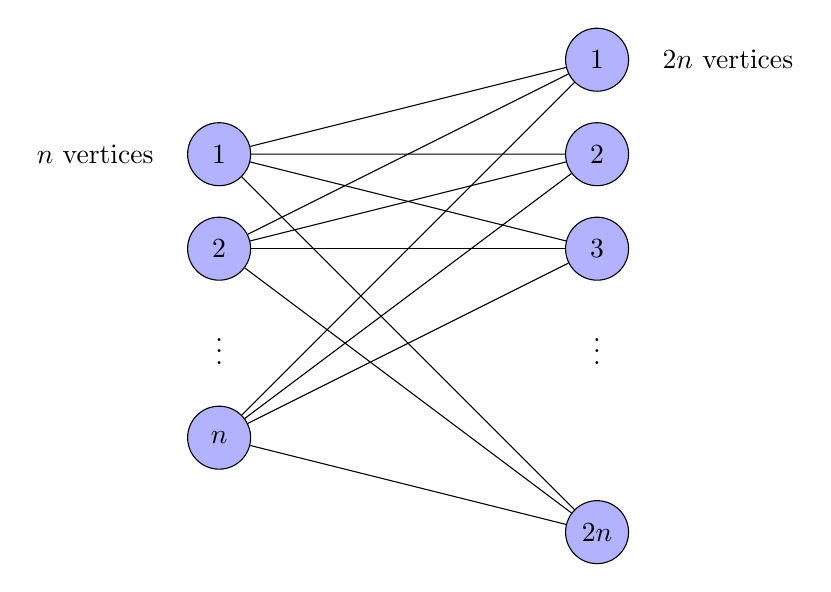
\begin{tikzpicture}[scale=1.2]

  % Left side (n vertices)
  \node[circle, fill=blue!30, draw, minimum size=8mm] (L1) at (0,2) {1};
  \node[circle, fill=blue!30, draw, minimum size=8mm] (L2) at (0,1) {2};
  \node at (0,0) {$\vdots$};
  \node[circle, fill=blue!30, draw, minimum size=8mm] (Ln) at (0,-1) {$n$};
  \node[left=3mm of L1] {$n$ vertices};

  % Right side (2n vertices)
  \node[circle, fill=blue!30, draw, minimum size=8mm] (R1) at (4,3) {1};
  \node[circle, fill=blue!30, draw, minimum size=8mm] (R2) at (4,2) {2};
  \node[circle, fill=blue!30, draw, minimum size=8mm] (R3) at (4,1) {3};
  \node at (4,0) {$\vdots$};
  \node[circle, fill=blue!30, draw, minimum size=8mm] (R2n) at (4,-2) {$2n$};
  \node[right=3mm of R1] {$2n$ vertices};

  % Example edges (schematic, not all drawn)
  \draw (L1) -- (R1);
  \draw (L1) -- (R2);
  \draw (L2) -- (R3);
  \draw (Ln) -- (R2n);
  \draw (L1) -- (R3);
  \draw (Ln) -- (R1);
  \draw (L1) -- (R2n);
  \draw (L2) -- (R1);
  \draw (L2) -- (R2n);
  \draw (Ln) -- (R2);
    \draw (Ln) -- (R3);
      \draw (L2) -- (R2);
  
\end{tikzpicture} ~\\
Call the left partite set $V_1$ and the right partite set $V_2$ and assume we have a Hamiltonian cycle $P: u_1,u_2,...,u_{3n},u_1$, then notice that every edge $u_i u_{i+1}$ must have one vertex in each partite set. But then for the $2n$ vertices in $V_2$, to each occur exactly once in $P$, there must be $2n$ vertices in $V_1$. But there is only $n$ vertices, so we cannot have a Hamiltonian path

Another counterexample is (using the cutting vertex component theorem):~\\
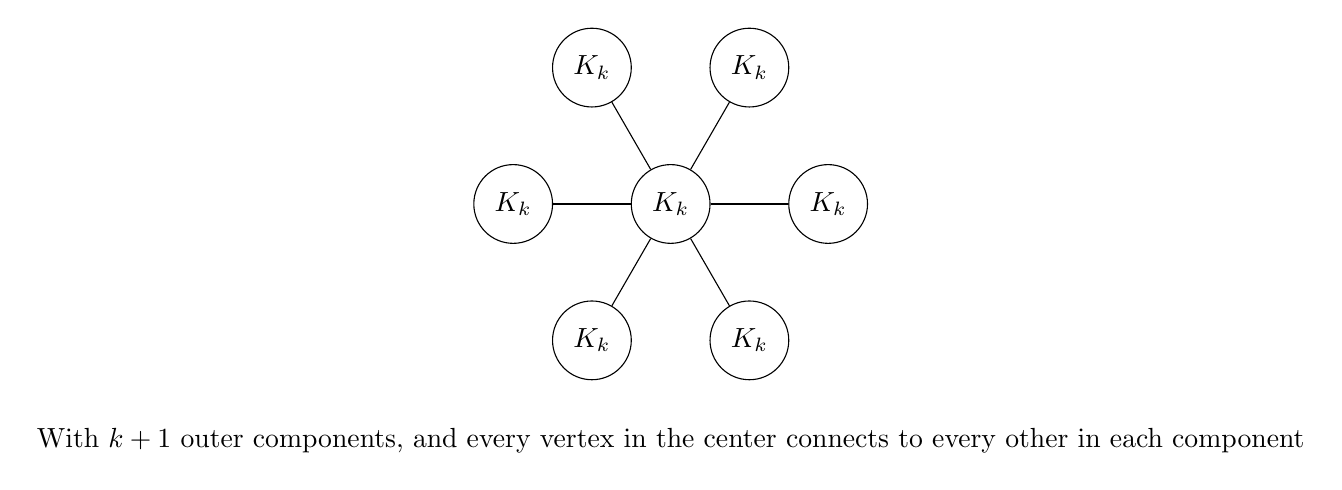
\begin{tikzpicture}[scale=2]

  % Central K_k
  \node[draw,circle,minimum size=1cm] (C) at (0,0) {$K_k$};

  % Place k+1 outer circles around in a circle
  \foreach \i in {1,...,6} { % example: k+1 = 6
    \node[draw,circle,minimum size=1cm] (O\i) at ({cos(60*\i)},{sin(60*\i)}) {$K_k$};
    \draw (C) -- (O\i);
  }

  % Label
  \node at (0,-1.5) {With $k+1$ outer components, and every vertex in the center connects to every other in each component};

\end{tikzpicture}

 \subsection*{Question 9: Prove that $\bar{C}_n$ is Hamiltonian for $n \ge 5$}
 In $C_n$, each vertex has degree $2$. In $\bar{C}_n$, every vertex has degree $(n-1)-2 = n-3$. For any non-adjacent vertices $u$ and $v$, we have that $\deg v + \deg u = 2n - 6 \ge n \iff n \ge 6$. It follows $\bar{C}_n$ is Hamiltonian for $n\ge 6$. The case $n=5$ is Hamiltonian with cycle $v_1, v_4, v_2, v_5, v_3, v_1$
 
 \begin{center}
 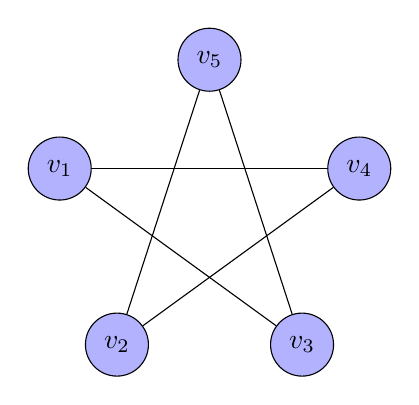
\begin{tikzpicture}[scale=2]
  % Place 5 vertices in a pentagon
  \foreach \i in {1,...,5}
    \node[circle, fill=blue!30, draw, minimum size=8mm] (v\i) 
      at (90+72*\i:1) {$v_\i$};
      
  % Draw the 5-cycle edges (complement of C5 is itself a C5)
  \foreach \i/\j in {1/3,2/4,3/5,4/1,5/2}
    \draw (v\i) -- (v\j);
\end{tikzpicture}
\end{center}


 
\subsection*{Question 10: Let $G$ be a 6-regular graph of order $10$ and let $u,v \in V(G)$. Prove that $G$, $G-u$, and $G-u-v$ are all Hamiltonian}
Let $x,y$ be nonadjacent vertices in:
\begin{itemize}
	\item  $G$. Then $\deg x + \deg y = 6+6 = 12 \ge 10$ so $G$ is Hamiltonian. 
	\item $G - u$. Then $\deg x + \deg y \ge 5 + 5 = 10 \ge 9$ so $G - u$ (a graph of order 9) is Hamiltonian (each vertex loses at most 1 edge)
	\item $G - u - v$. Then $\deg x + \deg y \ge 4 + 4 = 8$  so $G - u - v$ (a graph of order 8) is Hamiltonian (each vertex loses at most 2 edges)
\end{itemize}

 \subsection*{Question 11: The subdivision graph $S(G)$ of a graph $G$ is the graph obtained from $G$ by deleting every edge $uv$ of $G$ and replacing it by a vertex $w$ of degree $2$ that is joined to $u$ and $v$ (e.g., the subdivision graph of $C_3$ is $C_6$). Prove or disprove: If $S(G)$ is Hamiltonian, then $G$ is Eulerian}
 This is true. Let $G$ be a graph of order $n$. If $uv \in E(G)$, we will denote $x_{uv}$ as the new vertex in $S(G)$ such that $ux_{uv}$ and $x_{uv}v \in E(S(G))$. If $S(G)$ is Hamiltonian, we can find a Hamiltonian cycle $P:v_1, x_{v_1v_2}, v_2, x_{v_2v_3},v_3,...,v_n,x_{v_nv_1},v_1$ (since in $S(G)$, the only neighbours of a vertex $v \in G$ are the new $x_{uv}$ vertices for $u \in N(v)$ in $G$). Since this is Hamiltonian, every $x_{uv}$ is in the path. It follows that the path $v_1,v_2,...,v_n,v_1$ contains every edge. Since every vertex is occurs exactly once, every edge in $G$ occurs exactly once (there is a bijection between the $x$ vertices and edges). So $P$ is an Eulerian circuit making $G$ Eulerian

\subsection*{Question 12: A hamiltonian path is a path that contains every vertex of $G$, and a graph is traceable if it contains a hamiltonian path}
\subsubsection*{\ \ (a) Clearly, every hamiltonian graph is traceable. Is the converse true?}
No. Consider graph:

\begin{figure}[h]\centering
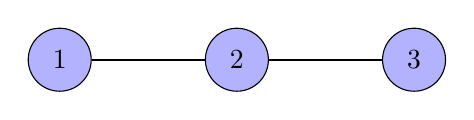
\begin{tikzpicture}[scale=1.5,
  every node/.style={circle, fill=blue!30, draw, minimum size=8mm}]
  
  \node (1) at (0,0) {1};
  \node (2) at (1.5,0) {2};
  \node (3) at (3,0) {3};
  
  \draw[thick] (1)--(2)--(3);

\end{tikzpicture}
\end{figure}
\subsubsection*{\ \ (b) Let $G$ be a graph of order $n\ge 3$ such that $\deg u + \deg v \ge n-1$ for every two nonadjacent vertices $u,v$ of $G$. Prove that $G$ is traceable}
Consider modifying graph $G$ into $H$ by adding a vertex $x$ and adding edges $ux$ for every $u \in V(G)$. Then $H$ is a graph of order $n+1$, and for every nonadjacent vertices $u$ and $v$, $\deg u + \deg v \ge n-1+2 = n+1$. So $H$ is Hamiltonian with cycle $P:v_1, v_2, ..., v_i, x, v_{i+1},...,v_n,v_1$. Then the path $v_{i+1}, ..., v_n, v_1, v_2, ..., v_i$ is a Hamiltonian path for $G$. So $G$ is traceable.

\newpage

\subsection*{Question 13: Let $G$ be a graph of order $n \ge 3$ having the property that for each $v \in V(G)$, there is a Hamiltonian path with initial vertex $v$. Show that $G$ is 2-connected but not necessarily Hamiltonian}
For every vertex $v$ in $G$, there is a path $P_v$ visiting every vertex, starting at $v$. Then starting at the next vertex is a path visiting every vertex in $G-v$, so $G-v$ is connected and thus $G$ is 2-connected. This graph need not be Hamiltonian, for example,
\begin{figure}[h]
\centering
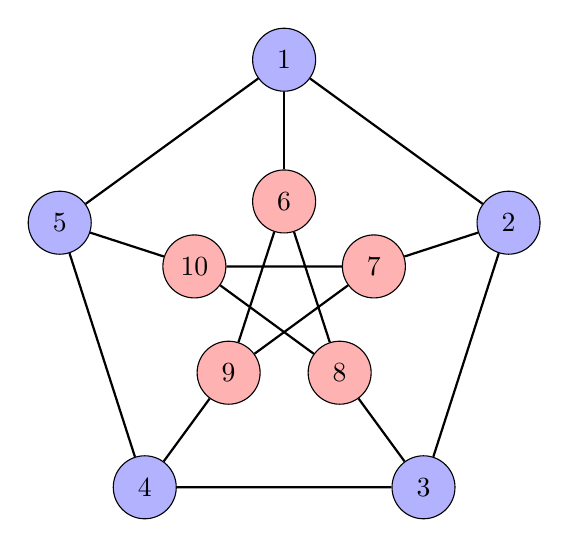
\begin{tikzpicture}[scale=1.5]
    % Outer pentagon vertices
    \node[circle, fill=blue!30, draw, minimum size=8mm] (O1) at (0,2) {1};
    \node[circle, fill=blue!30, draw, minimum size=8mm] (O2) at (1.9,0.62) {2};
    \node[circle, fill=blue!30, draw, minimum size=8mm] (O3) at (1.18,-1.62) {3};
    \node[circle, fill=blue!30, draw, minimum size=8mm] (O4) at (-1.18,-1.62) {4};
    \node[circle, fill=blue!30, draw, minimum size=8mm] (O5) at (-1.9,0.62) {5};
    
    % Inner pentagram vertices
    \node[circle, fill=red!30, draw, minimum size=8mm] (I1) at (0,0.8) {6};
    \node[circle, fill=red!30, draw, minimum size=8mm] (I2) at (0.76,0.25) {7};
    \node[circle, fill=red!30, draw, minimum size=8mm] (I3) at (0.47,-0.65) {8};
    \node[circle, fill=red!30, draw, minimum size=8mm] (I4) at (-0.47,-0.65) {9};
    \node[circle, fill=red!30, draw, minimum size=8mm] (I5) at (-0.76,0.25) {10};
    
    % Outer pentagon edges
    \draw[thick] (O1) -- (O2) -- (O3) -- (O4) -- (O5) -- (O1);
    
    % Inner pentagram edges (connecting every other vertex)
    \draw[thick] (I1) -- (I3) -- (I5) -- (I2) -- (I4) -- (I1);
    
    % Spokes connecting outer to inner
    \draw[thick] (O1) -- (I1);
    \draw[thick] (O2) -- (I2);
    \draw[thick] (O3) -- (I3);
    \draw[thick] (O4) -- (I4);
    \draw[thick] (O5) -- (I5);
    
\end{tikzpicture}
\caption{The Petersen Graph}
\label{fig:petersen}
\end{figure}

\subsection*{Question 14: If $G$ is a graph of order $n\ge 3$ with $\delta (G) \ge n/2$, prove that $G$ is Hamiltonian}
Let $u$ and $v$ be nonadjacent vertices. Then $\deg u + \deg v \ge \delta (G) + \delta (G) \ge n$. So $G$ is Hamiltonian 
\end{document}
